\documentclass[12pt, a4paper]{article}
\usepackage[utf8]{inputenc}
\usepackage[italian]{babel}
\usepackage{float}
\usepackage{newlfont}
\usepackage{hyperref}
\usepackage{multirow}
\usepackage{subfiles}
\usepackage{graphicx}
\usepackage{subfig}
\usepackage[toc,page]{appendix}

\textwidth=450pt\oddsidemargin=0pt
\graphicspath{ {./images/} }
\raggedbottom


\author{Marco Benito Tomasone 1038815 \\ 
        Luca Genova  1038843\\
 Master Degree in Computer Science\\}
\date{2022-2023}
\title{Network Analysis:\\ Network Structure and Team Performance: Euro 2020}

\begin{document}
\maketitle

\section{Abstract}
\label{abstract-not-needed-for-the-project-proposal}

Brief summary of the whole study (around 60-120 words), summarising the
salient parts of the sections below.

\section{Context}
\label{context}
Human interaction are very important in our society. In a lot of situations humans tend to group themselves in subset to operate in a more efficient way. Also in sports, humans organized themselves in teams to achive common goal and demostrate their skills and their ability to work in a group. In this case of interaction, the ways in which the members of the team interact with each other are more important, because the way people inside the team interact influence directly the results the team will obtain. In this study we will analyze the network structure of football teams and how it affects the performance of the team. In this work we focused on the last UEFA Euro 2020 tournament.
\subsection{Previous Work}
This work is heavely based on the work done by Thomas U. Grund in which he analyzed two seasons of the english Premier League. %TODO: add reference to the paper


%%%%%%%%
%The context includes: the general field (e.g., literature, history,
%archaeology, tourism, biology, forensics, religious studies); the
%specific application (e.g., literary analysis, quantitative history,
%genetics, virology, forensics intelligence, tourism planning, biblical
%quantitative studies).

\section{Problem and Motivation}
\label{problem-and-motivation}
In last year data science is a very growing field and this it's impacting a lot of different fields, sport included. In the football case, data are in most case an unknown technology and a lot of teams (even at highest level) don't use this type of knowledge to understand the performance of the team itself, but event of the opponents. Given that the way player interact each other can result in a better or worse performance of the team, it's important to understand how the network structure of the team can affect the performance of the team. 

%%%%%%%%%%%%%
%What are the problems you want to address? Why are those problems
%important (impact, theoretical and/ or practical needs, etc.)? What are
%the main contributions of the project?

\section{Datasets}
\label{datasets}
The data have been provided by StatsBomb, one the biggest provider for football data. The dataset is composed by every single event during the match: every pass, every shoot, every press and so on. 
The gathering process is based on a python library called StatsBombPy, which is a wrapper for the StatsBomb API. 
StatsBomb's Data are not for free, except for some free data, Euro 2020 is one of them. From StatsBombPy you get data in form of Pandas Dataframe, which is a very useful tool for data analysis. We used python and Pandas (a python library) to manage data and then we gathered data and store Data for all matches in .csv o .xlsx format. All other manipulation on data have been done using python and metrics have been computed using NetworkX (a python library for network analysis). The data we gathered contains all the matches of the tournament, so we have data for 51 matches. In a football match there are two team facing, so we have a total of 102 networks. We computed metrics for each network and then we analyzed the results.
%%%%%%%%%%%%%
%How did you gather the data? Did you digitise it? How? Is the material
%publicly available? What tools did you use 1) to handle (store,
%manipulate) the data and 2) to compute measures on the data?

\section{Validity and Reliability }
\label{validity-and-reliability-not-needed-for-the-project-proposal}
TODO: add validity and reliability
%%%%%%%%%%%%%%%%
%How closely does the model of your dataset represent reality (validity)?
%How consistent is the model you assembled (reliability)?


\section{Hypothesis}
Out work is based on two fundamental hypothesis:
\begin{enumerate}
        \item Team performance is affected by interaction opportunities: increased interaction intensity leads to increased team performance.
        \item Increased centralization of interaction in teams leads to decreased team performance.
\end{enumerate}
So the first hypothesis is based on the idea that the more a team interacts with each other, the more the team will be able to perform better. The second hypothesis is based on the idea that the more a team is centralized on a single player, the less the team will be able to perform better, because if a team makes to much reliance on a single player, the team will be more vulnerable to the opponent. 
\section{Measure}
\label{measures}
Based on the hypothesis we want to prove we focused on two metrics in particular:
\begin{itemize}
        \item Network Intensity
        \item Network Centralization
\end{itemize}
\subsection{Network Intensity}
Usually one of the most computed metrics of networks is density, which
is traditionally calculated as the number of existing ties in a network divided by the number of potential ties. In our case, we can't use this metric, because in a football match we can easily expect a pass between each pair of players in a team. So we need to define a new metric, which is weighted on the number of passes. To compute this new metric we need the information of the number of passes received and made by each player. So we used: 
\begin{itemize}
        \item \textbf{Out-strenght:} the number of passes made by the player $i$
        $$ C_{OS}(i) = \sum^{N}_{j=1}w_{ij}$$
        \item \textbf{In-strenght:} the number of passes received by the player $i$
         $$C_{IS}(i) = \sum^{N}_{j=1}w_{ji}$$
\end{itemize}
Where N is the number of nodes in the network, in our case is 11, because we consider only the starting XI of each team. We focused our attention on the starting XI instead of the best eight player for number of passes (as in Grund CITAAAAA) because we are analyzing a tournament. In a tournament in the final phase if two teams draw go to extra time so some player from the bench could impact the match in a more important way than others. To limit this problem we only focused on the starting XI. Another reason is that these tournament are very short (7 match at maximum) and the match are knockout game, so all the coach try to always play with the best players he has for that match. Another reason for which we focused only on the starting XI is that from 2020 the number of subs a coach can do is 5, while in the past it was 3 (that's because Grund used only the most eight players, because he ideally consider only the players who played the entire match). \\
So the network intensity for a team is defined as:
$$I = \frac{1}{T}\sum^N_{i=1} \frac{ C_{OS}(i) +  C_{IS}(i)}{2}$$
That is just the total number of passes made by a team in a match divided by the ball possession time in minutes. Given the data we had we can compute the effective ball possession time, so the sum of the time of possession of both team in a match does not sum up to 90 minutes, because in a match there are also the stoppages for injuries, substitutions, goals and so on. This can explain why the range of values the network intensity assumes in our case is slightly different from the one in Grund's paper.
\\
\subsection{Network Centralization}
The network centralization is computed by computing two different metrics: the weighted centralization and the strenght centralization. \\
\subsubsection{Weighted centralization}
The weighted centralization is one of the simplest way to examine the distribution of the weights in a network. It is defined as:
$$C_w = \frac{\sum^N_{i=1} \sum^N_{j=1} (w^* - w_{ij})}{(N^2 - N - 1)IT}$$
Where $w^*$ is the biggest tie value in the network (so the biggest number of passes between two players), $w_{ij}$ is the weight of the link between the node $i$ and the node $j$, $N$ is the number of nodes in the network (11) and $IT$ is the total number of passes of the team for that match. \\
This metric is zero in the  the most decentralized interaction pattern so when everybody interacts with everybody with the same intensity. In contrast, this metric is maximum (1) in the case the  most interactions involve the same two individuals. 
\subsubsection{Strenght centralization}
The streght centralization is used instead of the degree centralization, beacuse as said for the network density in (almost all) football matches we can expect a pass between each pair of players in a team. So we used a centralization for incoming and outcoming node strenght: 
$$C_I = \frac{\sum^N_{i=1}(C_{IS}^* - C_{IS}(i))}{(N - 1)IT}$$
$$C_O = \frac{\sum^N_{i=1}(C_{OS}^* - C_{OS}(i))}{(N - 1)IT}$$
Where $C_{IS}^*$ is the biggest incoming node strenght in the network (so the biggest number of passes received by a player), $C_{IS}(i)$ is the incoming node strenght of the node $i$, $C_{OS}^*$ is the biggest outcoming node strenght in the network (so the biggest number of passes made by a player), $C_{OS}(i)$ is the outcoming node strenght of the node $i$, $N$ is the number of nodes in the network (11) and $IT$ is the total number of passes of the team for that match. \\


%What measures did you apply (brief explanation of how they work)? How do
%they relate to the intent of the study? Why are they relevant?

\section{Results}
\subsection{Quantitative Analysis}
\label{quantitative-analysis}
We start the result section presenting a table summarising the results of the metrics we obtained for each of the 102 observation we made. \\
\begin{table}[h]
        \centering
        \begin{tabular}{|c|c|c|c|c|c|}
                \hline
                & Mean & Std\_dev & Min & Max & Obs \\
                \hline
                $I$  &  12.67415006 & 2.011584937 & 6.970118575 &16.65631825 &  102 \\
                \hline
                $C_w$  &  0.030206  &  0.011425 & 0.001864 & 0.065984 & 102 \\
                \hline
                $C_I$ & 0.073909 & 0.022539 & 0.032302 & 0.134383 & 102 \\
                \hline
                $C_O$ & 0.077249 & 0.022527 & 0.032 & 0.137046 & 102 \\
                \hline
        \end{tabular}
        \caption{Statistical summary of the metrics}
\end{table}

\subsection{Qualitative Analysis}
\label{qualitative-analysis}
\subsubsection{Pattern Recognition}
Analyze the network structure of a team give us a lot of information about the team's style of play and the way the coach organize the team in a particular match. We made a graphical visualization for each of the 102 observation we made, using a python library called \emph{mlpsoccer} and \emph{matplotlib}. We computed the average position of each player in the starting XI and we used this information to plot the network. The dimension of a node is proportional to the number of passes made by the player and the dimension of a edge is proportional to the strenght of that tie. Analyze these visualization give us a lot of insight. One of the most beautiful example we obtained is the network of the Spain against the Sweden. \\
%TODO: Change 
\begin{figure}
        \centering
        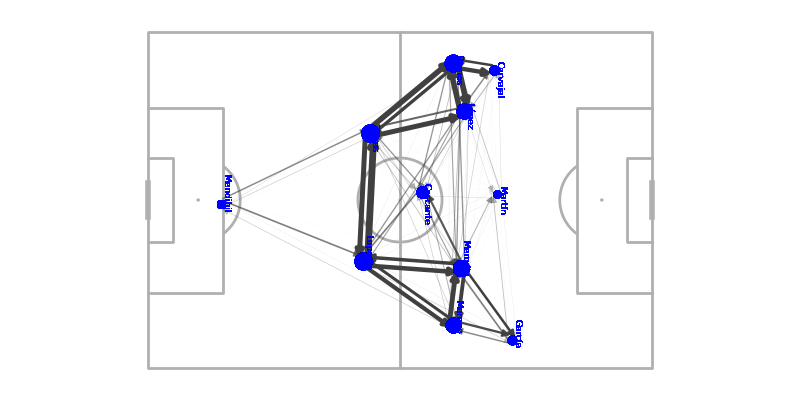
\includegraphics[width=0.8\textwidth]{../NoSubs/imgWithoutSubs/Spain_Network_Spain_Sweden.png}
        \caption{Spain-Sweden}
\end{figure}
As you can easily see this network is perfectly symmetric and this can make us recognize a pattern. This match is the most interesting example of the way the Spanish team plays, but starting from this, we can see that the Spanish team plays in a very similar way in almost all the matches. \\
\begin{figure}%
        \centering
        \subfloat[\centering Spain-Poland]{{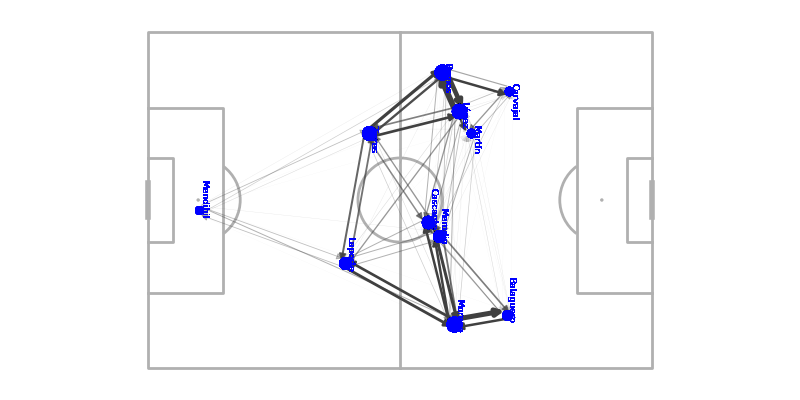
\includegraphics[width=0.4\textwidth]{../NoSubs/imgWithoutSubs/Spain_Network_Spain_Poland.png} }}%
        \qquad
        \subfloat[\centering Switzerland-Spain]{{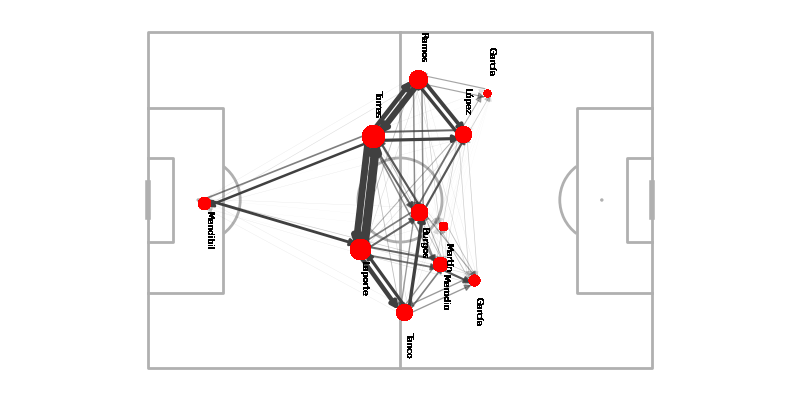
\includegraphics[width=0.4\textwidth]{../NoSubs/imgWithoutSubs/Spain_Network_Switzerland_Spain.png} }}%
        \label{fig:example}%
    \end{figure}

Other interesting example are the networks of Russia against Denmark and Poland against Spain. In these two matches the strongest tie between two players is a pass from the goalkeeper to the centre forward. This is due to the difference of quality between the two teams and the high pressing the two opponent team made during these matches, so the only playing possibility for Poland and Russia were to pass the ball to the goalkeeper and he had the only choice to make a long pass toward the striker. \\


\begin{figure}%
        \centering
        \subfloat[\centering Poland in  Spain-Poland]{{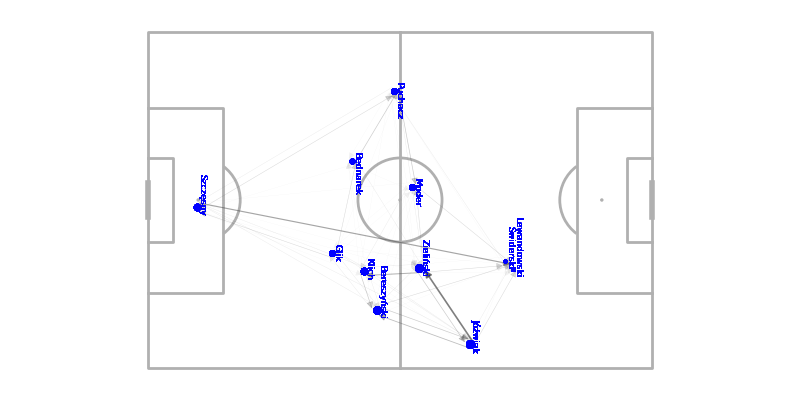
\includegraphics[width=0.4\textwidth]{../NoSubs/imgWithoutSubs/Poland_Network_Spain_Poland.png} }}%
        \qquad
        \subfloat[\centering Russia in Russia-Denmark]{{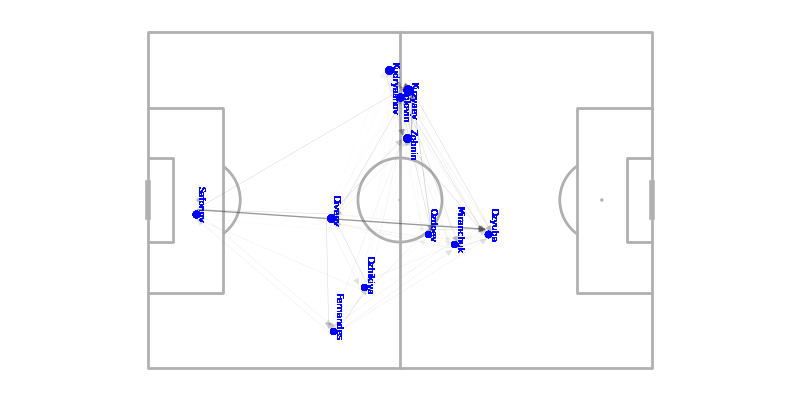
\includegraphics[width=0.4\textwidth]{../NoSubs/imgWithoutSubs/Russia_Network_Russia_Denmark.png} }}%
        \label{fig:example}%
    \end{figure}

\subsubsection{Node Centralization}
For each match, for each team we computed a weighted node centralization for each player. Then we computed the average weighted centralization for each player for each team. In some cases the results match our expectations, in other cases not. \\
The most evident example in which the difference between the average weighted centralization and the weighted centralization of a player is very high is the case of the Croatia team. As soon as Luka Modric (Croatia's captain) is one of the most important players in the world, and moreover in the football history, we did expect that he is the most important node in Croatia's networks. This hypothesis is totally confirmed as Modric is the node with the highest centralization in three on four matches played by Croatia in the tournament. The only match in which Modric is not the most important node in the network is the one against the Spain, in which the Croatia has been eliminated from the tournament losing 3-5. The reason behind the fact that in this match Croatia's captain was not the most important node is related with the high pressing Spain midfielders done on him on that match. This is a fantastic explanation of how analyze the network structure of a team can be very useful to gain information about the style of play of opponent teams and to make countermeasures.  \\ 
%%%%%%TABELLA SU MODRIC %%%%%%%%%%%
We expect to find the same result for the Portugal, as Cristiano Ronaldo is the most important player in the team. This is not the case, as the average weighted centralization of Ronaldo is lower than the weighted centralization of the other players. This is due to the fact that Ronaldo as a striker is not involved in the build-up of the play. The top two players for node centrality have been Ruben Dias and Pepe, the two centre back. This is the case of the majority of the teams for example Spain, England, France, Sweden, Ukraine and so on. This is due to the style of play of these teams: to retain the ball it is very usual to have a lot of passages between defenders. \\
An honour mention to the winner of the tournament: Italy. We did expect that Jorginho Frello would be the most important node in the Italian network, and dispite he is the most central node in just 2 matches on 7, he has the highest average weighted centralization, confirming our hypothesis. It is important to note that in the most matches the two most important nodes for Italy have always been Jorginho Frello or Marco Verratti, two midfielders. One important exceptions is the match against Spain (one of the most difficult match in the tournament for Italy) in wich the most important node has been Giorgio Chiellini, the centre back, for the same reason as Croatia-Spain. \\






%%%%%%%%%%%%%%%%%
%What is the connection among the gathered data, the applied measures,
%and the properties found?

\subsection{Conclusion (not needed for the project proposal)}
Qualitative analysis of the quantitative findings of the study.

\subsubsection{Critique (not needed for the project proposal)}
\label{critique-not-needed-for-the-project-proposal}

Do you think your work solves the problem presented above? To which
extent (completely, what parts)? Why? What could you have done
differently to answer your research problems (e.g., gather data with
additional information, build your model differently, apply alternative
measures)?

\end{document}
